\documentclass{beamer}

\mode<presentation> { \usetheme{Antibes} }

\usepackage{times}

\title{Version control systems}
\author{Finch \\
    The CAT
}

\AtBeginSection[]
{
    \begin{frame}<beamer>
	\frametitle{Outline}
	\tableofcontents[currentsection]
    \end{frame}
}

\begin{document}

\begin{frame}
    \titlepage
\end{frame}

\section{Introduction}

\begin{frame}
    \frametitle{What is VCS?}
    \begin{itemize}
	\item A Version Control System, or VCS, is a way to track changes to files
	\item Allows you to manage code or documents as you edit it
	\item Makes collaborating on a document/code significantly easier
    \end{itemize}
\end{frame}

\begin{frame}
    \frametitle{Why should you care?}
    \begin{itemize}
	\item Track changes to your files over time
	\begin{itemize}
	    \item Try out experimental ideas to code without risking any permanent harm
	    \item Use VCS on your homework to track your changes between drafts
	    \item Turn a VCS into a backup system!
	\end{itemize}
	\item Locate the revision that a bug was introduced
	\item Manage changes to a single file across multiple users
	\item VCS can prevent you from really buggering a project
	\begin{itemize}
	    \item ``Wait, you {\bf didn't} want that file deleted?''
	\end{itemize}
    \end{itemize}
\end{frame}

\begin{frame}
    \frametitle{Why should you care?}
    \begin{itemize}
	\item Any sane developer/project uses VCS
	\begin{itemize}
	    \item sourceforge
	    \item code.google.com
	    \item github/gitorious/git.or.cz
	\end{itemize}
	\item The CAT utilized VCS in many locations
	\begin{itemize}
	    \item agendas - RCS
	    \item CRACK - Git
	    \item intranet - Git
	\end{itemize}
    \end{itemize}
\end{frame}

\section{Background}

\begin{frame}
    \frametitle{Before VCS}
    \begin{itemize}
	\item Living dangerously!
    \end{itemize}
    vim foo.txt \\
    \begin{itemize}
	\item {\em three hours later} \\
    \end{itemize}
    rm *.txt \\
    \ldots \\
    \begin{itemize}
	\item Whoops. \\
    \end{itemize}
\end{frame}

\begin{frame}
    \frametitle{Do it yourself VCS}
    \begin{itemize}
	\item Users replicated VCS tools by doing everything by hand
    \end{itemize}
     vim foo.txt \\
     cp foo.txt foo.txt.1 \&\& vim foo.txt \\
     cp foo.txt.1 foo.txt.2 \&\& vim foo.txt \&\& cp foo.txt foo.txt.1 \&\& vim foo.txt \\
    \ldots
    \begin{itemize}
	\item Obviously, this is not a very fun idea
    \end{itemize}
\end{frame}


\begin{frame}
    \frametitle{The beginning of VCS}
    \begin{itemize}
	\item Initial idea of VCS came from engineering
	\item Engineers would create blueprints, and save earlier revisions
	\item If a version was not liked, it was trivial to roll back
	\item Revision control was also applied in business, law
	\item Any place where you may need to backtrack on a document, VCS will show up
    \end{itemize}
\end{frame}

\begin{frame}
    \frametitle{Concerns with VCS}
    \begin{itemize}
	\item Any VCS has to deal with some basic concerns
	\begin{itemize}
	    \item Merging changes
	    \item Locking files
	    \item Atomic commits
	\end{itemize}
	\item Each VCS handles these concerns differently
    \end{itemize}
\end{frame}

\section{File based VCS}

\subsection{SCCS}

\begin{frame}
    \frametitle{Source Code Control System (SCCS)}
    \begin{itemize}
	\item Arguably the first VCS system available
	\item Developed by Bell Labs in 1972
	\begin{itemize}
	    \item For some comparison, C was written in 1972 at Bell Labs as well
	\end{itemize}
	\item SCCS was the dominant VCS until the advent of RCS 
	\item Generally considered obsolete, and only mentioned for historical purposes
	\item Except for the storage method - still used today
    \end{itemize}
\end{frame}

\subsection{RCS}

\begin{frame}
    \frametitle{Revision Control System (RCS)}
    \begin{itemize}
	\item Released in 1982
	\item Created as an evolution of SCCS
	\item Stored changes of files as a series of diffs
	\item Very popular, still used today
    \end{itemize}
\end{frame}

\begin{frame}
    \frametitle{Pros and Cons of RCS}
    \begin{itemize}
	\item Advantages
	\begin{itemize}
	    \item Dirt simple
	    \item Only need to know a few commands
	    \item Changesets stored as series of diffs, so easy to view
	    \item File locking and branching supported
	\end{itemize}
	\item Disadvantages
	\begin{itemize}
	    \item Single files only
	    \item Cannot store entire projects
	    \item No security mechanisms - anyone can tamper with diffs
	    \item Branching sucks - everybody just locks the file
	    \begin{itemize}
		\item co -l agenda.dog
		\item vim agenda.dog
		\item ci -u agenda.dog
	    \end{itemize}
	\end{itemize}
    \end{itemize}
\end{frame}

\section{Centralized VCS}

\begin{frame}
    \frametitle{Modern VCS}
    \begin{itemize}
	\item While early VCS systems were an improvement, they were still lacking
	\item No real support for multiple users
	\item No support for project wide version control
	\begin{itemize}
	    \item Make changes in foo.c and bar.c, and changes in one break the other
	    \item No way to look at both of the changes without black magic and/or shell scripts
	\end{itemize}
	\item Technologies started coming out to deal with this 
    \end{itemize}
\end{frame}

\subsection{CVS}

\begin{frame}
    \frametitle{Concurrent Version Systems (CVS)}
    \begin{itemize}
	\item Behold! Another evolution!
	\item CVS was the first client-server VCS
	\item Instead of just hacking on one file in a specific location, you check out a project
	\item Support for project wide VCS
	\item Support for multiple users simultaneously working on one project
    \end{itemize}
\end{frame}

\begin{frame}
    \frametitle{Pros and Cons of CVS}
    \begin{itemize}
	\item Advantages
	\begin{itemize}
	    \item \ldots
	    \item I got nothing.
	\end{itemize}
    \item Disadvantages
	\begin{itemize}
	    \item Where do we start?
	    \item No moving/renaming of directories
	    \item No versioning of symbolic links
	    \item No unicode
	    \item No atomic commits 
	    \begin{itemize}
		\item It'll commit enough changes to break everything!
	    \end{itemize}
	    \item CVS was used because it was the first, not because it was good.
	\end{itemize}
    \end{itemize}
\end{frame}

\subsection{SVN}

\begin{frame}
    \frametitle{Apache Subversion (SVN)}
    \begin{itemize}
	\item Since CVS sucked so much, people wanted an alternative
	\item SVN was designed as CVS without the problems
	\item Widely adopted by the open source community
	\item Support for a wide number of features
    \end{itemize}
\end{frame}

\begin{frame}
    \frametitle{SVN Features}
    \begin{itemize}
	\item Support for Properties
	\begin{itemize}
	    \item On the fly keywording in the source - note the last changed date in a comment
	    \item Store mime-types
	    \item Store executable bit (*nix)
	\end{itemize}
    \item Sane branching
    \item Support for authentication/authorization
    \item Atomic commits
    \item Sane file locking
    \end{itemize}
\end{frame}

\begin{frame}
    \frametitle{Example SVN structure}
    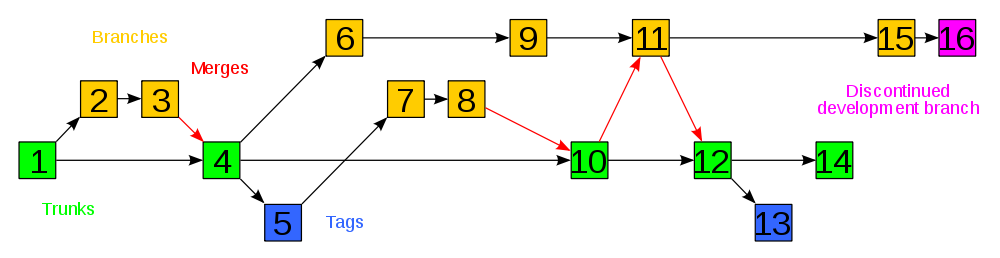
\includegraphics[scale = 0.30]{images/Subversion_project_visualization.png}
\end{frame}

\begin{frame}
    \frametitle{Pros and Cons of SVN}
    \begin{itemize}
	\item Advantages
	\begin{itemize}
	    \item The most widely used VCS today
	    \item Robust and battle tested
	    \item Fully centralized - collaboration is very easy
	    \item Support for branching and tagging
	\end{itemize}
	\item Disadvantages
	\begin{itemize}
	    \item Fully centralized - no offline work
	    \item Slow - network latency can increase time to work
	    \item Based on CVS
	\end{itemize}
    \end{itemize}
\end{frame}

\section{Decentralized VCS}

\begin{frame}
    \frametitle{Decentralized VCS}
    \begin{itemize}
	\item Centralized VCS has many limitations
	\begin{itemize}
	    \item No offline work
	    \item Forking a project is not trivial
	    \item Centralized model is not always the best for a project
	\end{itemize}
	\item People started experimenting with a decentralized model
    \end{itemize}
\end{frame}

\begin{frame}
    \frametitle{Differences between CVCS and DCVS}
    \begin{itemize}
	\item Differences
	\begin{itemize}
	    \item All working copies are branches
	    \item Most actions are local;
	    \item Central repository can exist, but is not required
	\end{itemize}
	\item Advantages
	\begin{itemize}
	    \item Easy to fork and merge code
	    \item Network connectivity is not required to use DVCS
	    \item Resistant to failure
	\end{itemize}
	\item Disadvantages
	\begin{itemize}
	    \item Initial clone is costly, as it copies the entire repo
	    \item Added complexity 
	\end{itemize}
    \end{itemize}
\end{frame}

\begin{frame}
    \frametitle{List of DVCS tools}
    \begin{itemize}
	\item Arch
	\item Monotone
	\item Darcs
	\item Bazaar
	\item Mercurial
	\item {\bf Git} (We like git)
    \end{itemize}
\end{frame}


\subsection{Git}

\begin{frame}
    \frametitle{Introduction to Git}
    \begin{quotation}
    ``I'm an egotistical bastard, and I name all my projects after myself. First Linux, now git.'' \\
    - Linus Torvalds
  \end{quotation}
    \begin{itemize}
	\item Git is the heavyweight of the DVCS world
	\item Open source DVCS created by Linus Torvalds, creator of the Linux kernel
	\item Created to fill the gap left by a previous proprietary DVCS
	\item The result of letting kernel hackers write a DVCS
    \end{itemize}
\end{frame}

\begin{frame}
    \frametitle{The inspiration for Git}
    \begin{itemize}
	\item Git is a remarkable tool that had to fulfill a difficult set of obligations
	\item Track the entire kernel history, with incredible amounts of information
	\item Needed to be small, fast, and powerful
	\item Designed to be the complete opposite of CVS
    \end{itemize}
\end{frame}

\begin{frame}
    \frametitle{Characteristics of Git}
    \begin{itemize}
	\item Designed for nonlinear development (Think kernel development)
	\item Built for distributed and offline work
	\item Built for speed and ability to handle large projects
	\item Cryptographic authentication/verification
    \end{itemize}
\end{frame}

\subsubsection{Git internals}

\begin{frame}
    \frametitle{Implementation}
    \begin{itemize}
	\item Written in C
	\item More closely resembles a filesystem than a standard VCS
	\begin{itemize}
	    \item This is what happens when you let a kernel hacker write a VCS!
	\end{itemize}
	\item Has types of blob, tree, commit, and tag
	\item Objects are identified by a SHA-1 hash
    \end{itemize}
\end{frame}

\begin{frame}
  \frametitle{Why hash everything?}
  \begin{itemize}
    \item Using hashes to identify parts of git repository may seem bizarre, but it adds a lot to git
    \item Hashes ensure that nobody can tamper with any part of the repository without changing hashes
    \item Allows for super fast retrieval of files
      \begin{itemize}
	\item Instead of searching a series of files for some content, you look for a specific filename
	\item Instead of slowing down git, using hashes speeds it up
      \end{itemize}
  \end{itemize}
\end{frame}

\begin{frame}
    \frametitle{Blob}
    \begin{itemize}
      \item A ``blob'' is used to store file data - it is generally a file.
      \item Only contains the contents of a file 
      \item No attributes like the file name are stored
    \end{itemize}
    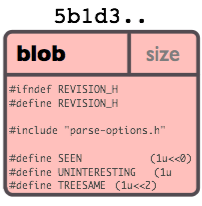
\includegraphics{images/object-blob.png}
\end{frame}

\begin{frame}
    \frametitle{Tree}
    \begin{itemize}
      \item A ``tree'' is basically like a directory 
      \item It references a bunch of other trees and/or blobs (i.e. files and sub-directories)
    \end{itemize}
    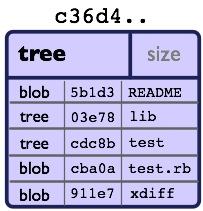
\includegraphics{images/object-tree.png}
\end{frame}

\begin{frame}
    \frametitle{Commit}
    \begin{itemize}
      \item A ``commit'' points to a single tree, marking it as what the project looked like at a certain point in time. 
    \end{itemize}
    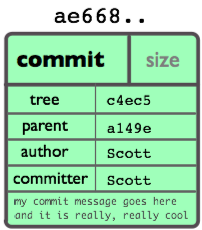
\includegraphics{images/object-commit.png}
\end{frame}

\begin{frame}
    \frametitle{Tag}
    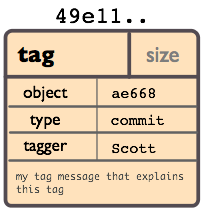
\includegraphics{images/object-tag.png}
\end{frame}

\begin{frame}
    \frametitle{Example}
    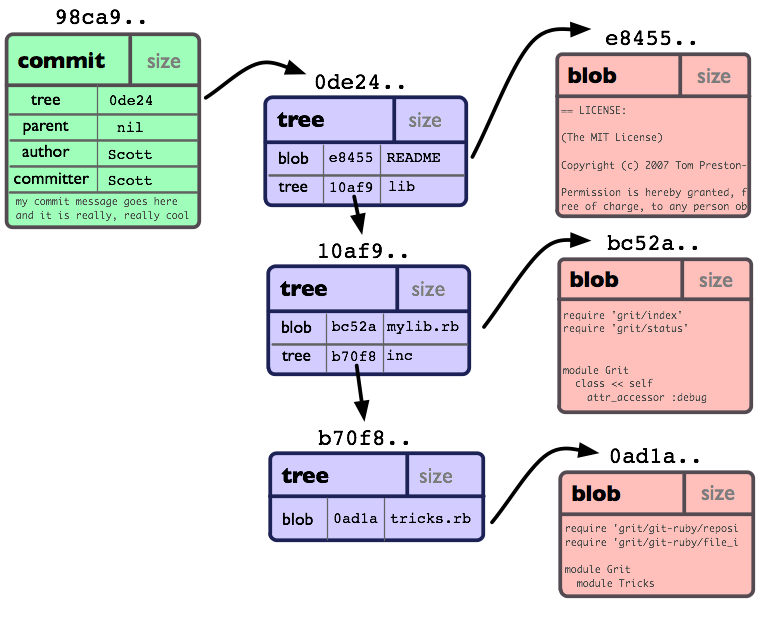
\includegraphics[ scale = .50 ]{images/objects-example.png}
\end{frame}

\subsubsection{Using Git}

\begin{frame}
    \frametitle{Git workflow}
    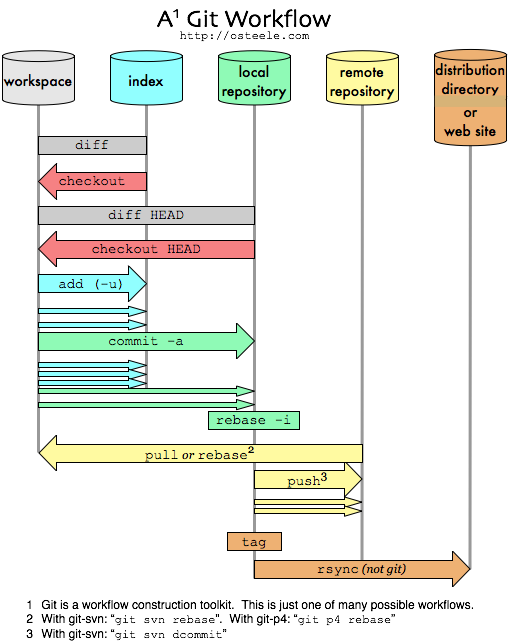
\includegraphics[scale = 0.3]{images/git-workflow.png}
\end{frame}

\begin{frame}
    \begin{itemize}
	\item Demo time!
    \end{itemize}
\end{frame}

\end{document}

